\begin{section}{The Irrationality of $\sqrt{2}$}

In this section\footnote{This section is derived from work of \href{http://users.dickinson.edu/~richesod/}{Dave Richeson} of Dickinson College.} we will prove one of the oldest and most important theorems in mathematics. The Pythagoreans were an ancient secret society that followed their spiritual leader: Pythagoras of Samos (c.\ 570-495 BCE). The Pythagoreans believed that the way to spiritual fulfillment and to an understanding of the universe was through the study of mathematics. They believed that all of mathematics, music, and astronomy could be described via whole numbers and their ratios. In modern mathematical terms they believed that all numbers are rational. Attributed to Pythagoras is the saying, ``Beatitude is the knowledge of the perfection of the numbers of the soul.'' And their motto was ``All is number.''

Thus they were stunned when one of their own---Hippasus of Metapontum (c.\ 5th century BCE)---discovered that the side and the diagonal of a square are incommensurable. That is, the ratio of the length of the diagonal to the length of the side is irrational\footnote{Recall that a number is \textbf{rational} if it can be written in the form $\frac{m}{n}$, where $m,n\in\mathbb{Z}$ and $n\neq 0$.  A number is \textbf{irrational} if it is not rational.}. Indeed, if the side of the square has length $a$, then the diagonal will have length $a\sqrt{2}$; the ratio is $\sqrt{2}$ (see Figure~\ref{fig:square}).  In today's language, Hipassus discovery is given by the following theorem.

\begin{figure}[ht]
\begin{center}
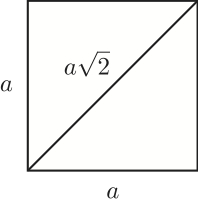
\includegraphics{square.png}
\end{center}
\vspace{-.5cm}
\caption{The side and diagonal of a square are incommensurable.}
\label{fig:square}
\end{figure}

Before tackling a proof of Theorem~\ref{thm:sqrt2}, we need a few tools.  In particular, we will make use of the Fundamental Theorem of Arithmetic (see Corollary~\ref{cor:FTA}).  The following result makes up half of the Fundamental Theorem of Arithmetic.

\begin{theorem}\label{thm:prodprimes}
Let $n$ be a natural number greater than 1.  Then $n$ can be expressed as a product of primes.  That is, we can write
\[
n=p_1 p_2 \cdots p_k,
\]
where each of $p_1, p_2, \ldots, p_k$ are prime numbers (and there may possibly be repeats in this list).\footnote{\emph{Hint:} Use a proof by contradiction.  Let $n$ be the smallest natural number for which the theorem fails.  Then $n$ cannot be prime since this would satisfy the theorem.  So, it must be the case that $n$ has a divisor other than 1 and itself.  This implies that there exists natural numbers $a$ and $b$ greater than 1 such that $n=ab$.  Since $n$ was our smallest counterexample, what can you conclude about both $a$ and $b$?  Use this information to derive a counterexample for $n$.}
\end{theorem}

The previous theorem states that we can write every natural number as a product of primes, but it does not say that the primes and the number of times the primes appear are unique.  It turns out that this is fairly difficult to prove.  We will need the following result known as the Division Algorithm, but we won't worry about proving it.  Instead, we will take it for granted and use it in the proof of Theorem~\ref{thm:Euclid}, which we will then use to prove uniqueness.

\begin{theorem}[Division Algorithm]
Suppose that $m,n\in\mathbb{N}$.  Then there exists unique $q,r\in\mathbb{N}$ such that $m=nq+r$ with $0\leq r<n$.
\end{theorem}
The numbers $q$ and $r$ from the Division Algorithm are referred to as \textbf{quotient} and \textbf{remainder}, respectively.  Now, see if you can prove the following theorem, which is known as Euclid's Lemma.

\begin{theorem}[Euclid's Lemma]\label{thm:Euclid}
Assume that $p$ is prime.  If $p$ divides $ab$, where $a,b\in\mathbb{N}$, then either $p$ divides $a$ or $p$ divides $b$.\footnote{\emph{Hint:} Use a proof by contradiction and apply the Division Algorithm to both $a$ and $b$.  What can you say about $ab$?}
\end{theorem}

Alright, let's tackle the uniqueness of the product of primes now.

\begin{theorem}\label{thm:unique}
Let $n$ be a natural number greater than 1.  Then the expression for $n$ as the product of one or more primes is unique (up to the order in which they appear).\footnote{\emph{Hint:} Use a proof by contradiction.  Write $n$ as both $p_1 p_2 \cdots p_k$ and $q_1 q_2 \cdots q_l$, where both are products of primes.  Use Euclid's Lemma to derive a contradiction.}
\end{theorem}

The following corollary follows immediately from Theorem~\ref{thm:prodprimes} and Theorem~\ref{thm:unique}.

\begin{corollary}[Fundamental Theorem of Arithmetic]\label{cor:FTA}
Every natural number greater than 1 can be expressed uniquely (up to the order in which they appear) as the product of one or more primes.
\end{corollary}

We are finally ready to prove that $\sqrt{2}$ is irrational.

\begin{theorem}
\label{thm:sqrt2}
The real number $\sqrt{2}$ is irrational.\footnote{\emph{Hint:} Use a proof by contradiction.  That is, suppose that there exist $m,n\in\mathbb{Z}$ such that $n\ne 0$ and $\sqrt{2}=\frac{m}{n}$. Next, square both sides and solve for $m^2$. How many factors of 2 does $m^2$ have?  How many factors of 2 does $2n^2$ have? Derive a contradiction using Corollary~\ref{cor:FTA}.}
\end{theorem}

As one might expect, the Pythagoreans were unhappy with this discovery. Legend says that Hippasus was expelled from the Pythagoreans and was perhaps drowned at sea. Ironically, this result, which angered the Pythagoreans so much, is probably their greatest contribution to mathematics: the discovery of irrational numbers.

Now, let's tackle a few more problems dealing with irrational numbers.

\begin{problem}
Determine whether $\displaystyle \frac{1+\sqrt{2}}{3+2\sqrt{2}}$ is rational or irrational and then prove that your answer is correct.
\end{problem}

\begin{theorem}\label{thm:sqrtp}
Let $p$ be a prime number.  Then $\sqrt{p}$ is irrational.
\end{theorem}

\begin{exercise}
Let $p$ be a prime number.  For which values of $n\in\mathbb{N}$ is $\sqrt[n]{p}$ irrational?  You do not need to prove your answer.
\end{exercise}

\begin{theorem}\label{thm:sqrt(pq)}
Let $p$ and $q$ be distinct primes.  Then $\sqrt{pq}$ is irrational.
\end{theorem}

\begin{problem}
State a generalization of Theorem~\ref{thm:sqrt(pq)} and briefly describe how its proof would go.  Be as general as possible.
\end{problem}

\begin{remark}
It is important to point out that not every positive irrational number is equal to the square root of some natural number.  For example, $\pi$ is irrational, but is not equal to the square root of a natural number.
\end{remark}

It is worth pointing out that our approach for proving that $\sqrt{2}$ was irrational was not the most efficient.  However, our technique was easy to generalize to handle results like Theorem~\ref{thm:sqrtp}.

\end{section}